\chapter{Conclusions}
\label{Chapter7}
\lhead{Chapter 7. \emph{Conclusions}}

\begin{figure}[H]
  \centering
  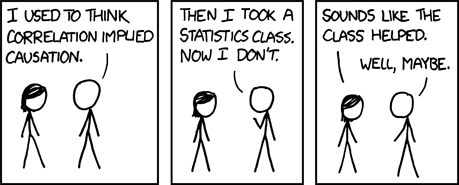
\includegraphics[width=0.6\textwidth]{Figures/xkcd/chapter7.png}
  \caption*{xkcd.com/552}
\end{figure}

In this thesis I have aimed to demonstrate the ability to photometrically classifing SLSNe amongst large samples of transients detected by modern, wide-field astronomical surveys. In order to achieve this, I have combined our understanding of this class of objects with state-of-the-art Machine Learning and light curve modelling techniques to both define and predict their behaviour in a number of surveys. All this was performed with the aim of broadening our understanding of SLSNe as a population. The main results are summerised below.

\section{Modelling SN light curves}
In \cref{Chapter3}, I described the methods for modelling of CCSN and SLSN. I discussed both the analytical models as well as the the tools built to implement them. Furthermore, I described the Bayesian approach to the problem of model optimisation and introduces Gaussian Processes as a tool for non-parametric, probabilistic light curve interpolation.

\subsection{Modelling SLSNe}
The simulations of SLSNe at any redshift or bandpass were essential for this thesis. In \sref{sec:SLAP}, I demontrated an approach to producing a high quality SLSN SED model based on the black-body approximation of its continuum, combined with a spectral absorption template. The templates, focusing on the UV regions of the SED, significantly increased the redshift range at which I could confidently model these objects. I combined this with the evolution of the bolumetric luminosity of SLSNe based on the birth and spin-down of a magnetar model, modified to include a variable opasity term. I showed that this treatment of SLSNe correctly accounts for their light curve morphonogy including the late time evolution which is difficult to capture using other models.

\subsection{Modelling CCSN}
While CCSN are a better understood class of transients than SLSNe, their simulation tools are still lacking, specially in comparison to SN\,Ia. Here, I developed a set of tool for the modelling and simulations of CCSNe including both their hydrogen poor and rich subclasses. I provide a self contained solution, beginning with the archival photometry and spectroscopy for a number of nearby objects. Using an approach similar to \citet{Bazin2009}, I model their light curves in order to provide an interpolation model used to flux calibrate the observed spectra in the process refered to as mangling. Based on this approach, I built CoCo, a tool for generating spectral templates as well as using them to simulate these SNe.

The simulations work on a principle of placing the spectral template at any required redshift, then passing it through a bandpass filter, measuring the synthetic flux at the phases of the spetra, before fitting a light curve model to them to obtain flux at any arbitrary point in the light curve. Due to the wavelength limitations of ground based spectroscopy, the SED had to be extended in both IR and UV regimes. I used a combination of auxillary \textit{Swift}-UVOT data and the modelling of their continuum as dust extincted black-bodies to achieve a wavelength coverage down to $\sim1500\AA$, sufficient to measure the flux of a CCSN in the DES \textit{g}-band at their detection limit of z$\sim$0.7.

\subsection{Light Curve interpoaltion using Gaussian Processes}
One of the greatest challenges I have overcome in this thesis was the problem of interpolating light curves of all generic transient. Using GPR, I developed a method which allowes me to generate a probabilistic interpolation for any light curve without introducing analytical models that bias the results by correlating all data points using a functional form. Throughout this thesis, I used the \Mate\'rn 3/2 kernel to model the covariance function of the data as I found it to be the best overall match to the typos of transients detected by DES.

\section{Rates of SLSN}
\cref{Chapter4} of this thesis focused on measuring the rate of SLSNe at the intermediate redshift of z$\sim$1. This was motivated by the low numbers of similar measurements, despite being a crucial piece of the puzzle of the origin on SLSNe. I provided one of the most accurate measurements of the rate, allowing us for the first time to probe the its evolution with redshift as well as the connection to other rare classes of transients.

\subsection{Defining SLSNe}
Starting from the SLSN models, based on the spin-down of a magnetar, I postulated a definition the SLSNe. After fitting the literature sample of these objects with the model, I found that SLSN concentrate in a small region of the P$_{ms}$-B$_{14}$-$\mathrm{\tau}_M$ parameter space, clearly separated from a majority of transients detected my the SNLS. I parametrised this region using an ellipsoid that tightly encapsules the entire training sample, giving a definition of a SLSN in terms of the parameter space of the magnetar model.

\subsection{Search for SLSN in SNLS}
I used my proposed definition of SLSNe to search for the presence of new, previosly unclassified SLSNe in the SNLS. Upon fittin its entire archival sample of transients, taking either their precise spectroscopic redshift (where available) or a range of host galaxy photometric redshift estimates I find that only two new objects fall within my definition. While one of the objects shows signs of multiseason variability, the second object, SNLS07D3bs, was found to be a strong SLSN candidate. My modelling suggested a good match to the class at 0.6$<$z$<1$. Using a low Sn\/N, archival spectrum of the object we were unable to confirm the classifcation, however, we used narrow line features to determine the true redshift of the object as z=0.74, confirming the object to be consistent with a luminosity of a SLSN.

\subsection{Rate of SLSNe at z$\sim$1}
With three SLSN candidates found in the SNLS, I performed a Monte Carlo simulation of the survey, replicating its transient detection behaviour. This reversed the common approach of calculating the rate of SNe by weighing each objects by its detection efficiency and observed volume. Instead, I simulated SLSNe before applying the survey noise and measuring each objects detectibility in the survey. Throughout the simulation, I iterate over a range of rate values to measure the resulting number of simualated detections. I then transpose these results to give me the probability of detecting 3 objects as a function of the input value. I found the rate of SLSNe at z$\sim$1 to be $91^{+76}_{-36}$\,SNe\,Yr$^{-1}$\,Gpc$^{-3}$ or 2.2$^{+1.8}_{-0.9}\times10^{-4}$ of the CCSN rate. This is consistent with similar pulications and tentitively demonstrates that the rate of SLSNe follows that of the star formation rate of the universe.

\subsection{Connection between SLSNe and ULGRBs}
An interesting question that we probed in \citet{Prajs2016} is the connection between the class of SLSNe and ULGRBs. LGRB are known to be connected to ordinary, stripped-envelope SNe as they result in the formation of a collapsar, or a jet forming young black hole powered by the infalling ejecta. Thanks to the advances in GRB observation provided by the \textit{Swift} satellite, we now know that some LGRB are observed to emmit $\gamma$-radiation for up to 10,000s. Classified as ULGRB, these events are known to be rarer than than ordinary LGRBs with their exact rate difficult to estimate due to the design of \textit{Swift}.

The discovery of an ULGRB, GRBXXXX introduced us to a potential connection to SLSNe as the object was observed as SN2011kl, an SN with a luminosity and monrphology similar to that of a number of lower luminosity SLSNe. It was also shown to have very similar spectroscopic characteristics.

\section{Photometic classification of SN}
Photometric classification of SNe forms the center piece of this thesis. Performed using a number of method, I demonstrate that the ML apprach is by far the most powerful approach to the problem, albeit, not the most straightforward to implement. While it required the construction of a large, artificial training sample, the results obtained using this method have largely exceeded the capabilities of other tools publically available to date. 

\subsection{Training sample}
Using the models of readily available models for SN\,Ia and AGNs, custum build models of SLSNe and CCSN, DES noise models and data augmentation using GPR, I have build a large training sample of SN matching the properties of the the real DES transient sample. Consisting $\sim$300,000 object, this is the largest to date light curve sample used for a photometric classification study and represents objects from the edge of detectibility by DES to local objects.

\subsection{Machine Learning Model}
In order to optimise the classification process, the machine learning models have been divided into two classes. First I worked to create a pure sample of SN-like events in combining the samples of various SN subclasses into a single label classified against the smaple of AGN and spurious survey noise. This produces a classification rate of 99.81\%, as measured on the subsample of the training data, as was further validated using the ground-truth sample of spectroscopically confirmed SLSNe which were all correctly identified in this work.

Upon the identification of a sample of DES SN, consiting of 5273 objects, I attemted to subclassify these objects using only SN light curves as the labeled training set. This again produces a strong classification model, capable of correctly identifying nearly all spectroscopically confirmed SN\,Ia. Applying this to the sample of DES transients I found 500 SLSN candidates, a number which vastly exceeds our expectations based on the rate measured in \cref{Chapter4}. Visual instection of the data showed that the sample is heavily contaminated by SN\,IIP which lacked in our training sample due to the low quality of their available spectral series.

\section{Selecting SLSN}
text

\section{Future Work}
text

\subsection{Expanding the Training Sample}
text

\subsection{Rates of SLSNe from DES}
A natural extention of the work undergone in Chapters \ref{Chapter4}-\ref{Chapter6} is to compute the rate of SLSN using this new and expanded sample of objects. The improvement from 3 to XX objects alone will result in a vastly descred uncertainties in the overall rate of SLSNe. However, more importantly it will be the first ever measurement that will allow for a separation of the rate into separate reshift bins using a homogeneus sample.

....

\subsection{Selecting SLSN in LSST}
The upcoming decad

\subsection{Redshift estimation for photometric SN\,Ia in DES}
Perhaps one of the most interesting results of this thesis, not directly related to its main subject of SLSNe, is the accuracy of photometric selection of SN\,Ia that was obtained purely as a by product of the main analysis. It is worth noting here that the model used for SN\,Ia only included cosmologically
